\begin{comment}
A similar study was applied to Natural Language metrics~\cite{readable}, which were calculated for each question. As many metrics were proposed, we must assemble a variable reduction, again to prevent an overspecific model. We started by assessing the normality of the given metrics, using a Kolmogorov-Smirnov test. The results in Figure~\ref{fig:02_ks_nlmetrics} indicates that the majority of the proposed Natural Language metrics do not follow a normal distribution, D(140) = .089, p = .009 (for Flesch–Kincaid Grade Level metric, other metrics show similar results).

\begin{figure}[!h]
\centering
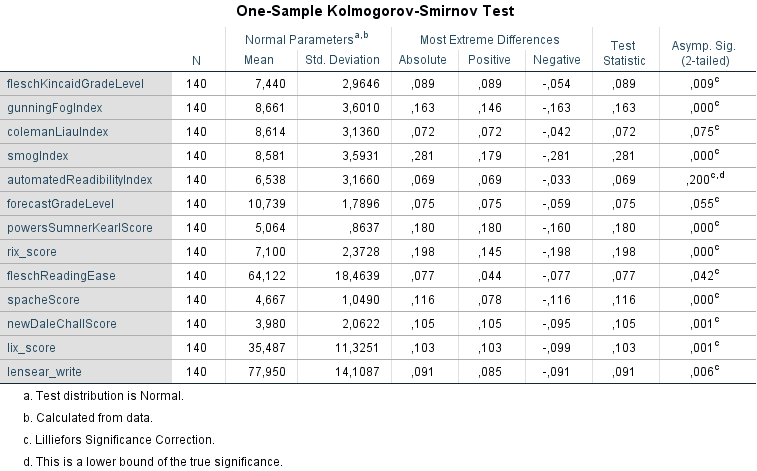
\includegraphics[width=1\textwidth]{figures/6_Results/Section2/02_KS_NLmetrics}
\caption{Kolmogorov–Smirnov test on the normal distribution of Natural Language metrics (English)}
\label{fig:02_ks_nlmetrics}
\end{figure}

To evaluate if the complexity of Natural Language (questions) can explain the success of students answers, and because the independent variables (metrics) don't follow a normal distribution, we applied a Spearman's rho correlation coefficient to evaluate their correlation, and their effect on the dependent variable (student's success). Figure~\ref{fig:02_sr_nlmetrics} presents the result of this assessment. We decided to exclude metrics with strong correlation (painted with red), as they can be used to explain the same results and keep the ones that are more dissimilar. The resulting metrics were the Automated Readability Index, Forest Grade Level, New Dale-Chall, and Lensear Write, as they revealed greater influence on the dependent variable.

\begin{figure}[!h]
\centering
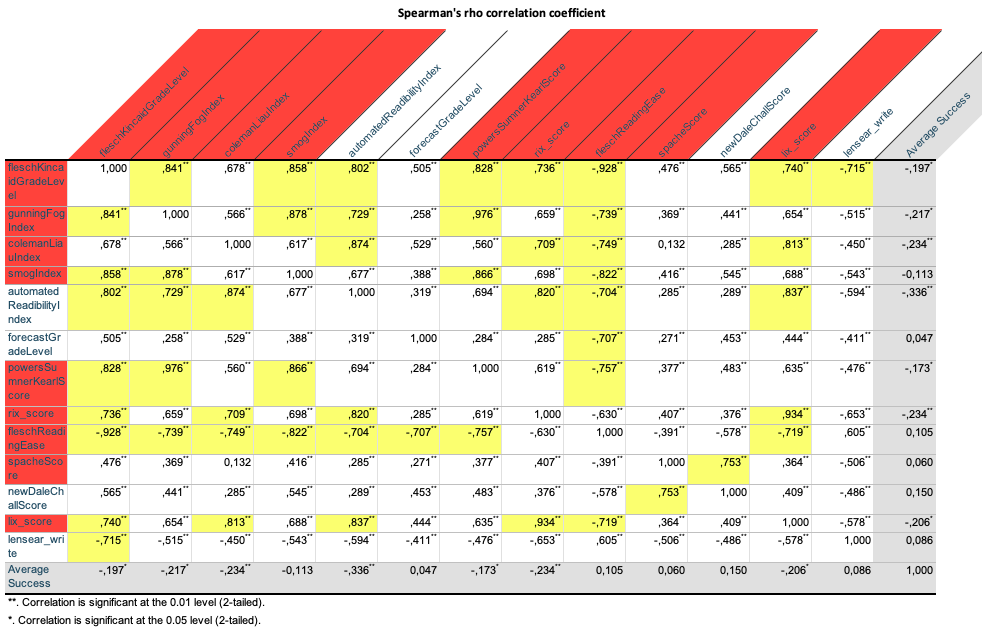
\includegraphics[width=1\textwidth]{figures/6_Results/Section2/02_SR_NLmetrics}
\caption{Spearman's rho correlation coefficient of NL metrics (English)}
\label{fig:02_sr_nlmetrics}
\end{figure}

The results of the regression on Natural Language metrics are shown in Figure~\ref{fig:02_lr_nlmetrics}. A significant regression equation was found F(4, 135) = 6.311, $p<.001$, with an $R^{2}$ of .158.

\begin{figure}[!h]
\centering
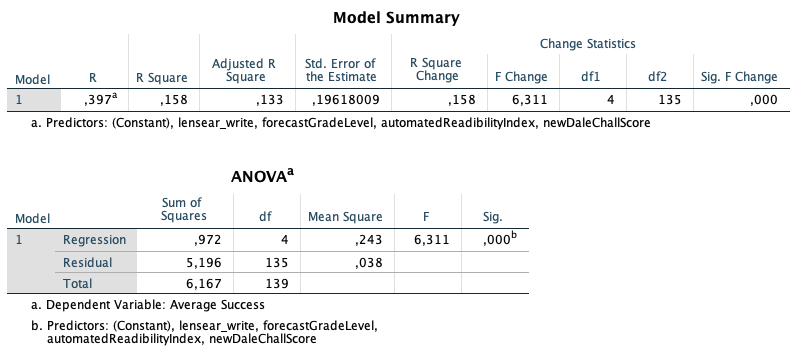
\includegraphics[width=1\textwidth]{figures/6_Results/Section2/02_LR_NLmetrics.png}
\caption{Linear Regression using Automated Readability Index, Forest Grade Level, New Dale-Chall, and Lensear Write to explain the success}
\label{fig:02_lr_nlmetrics}
\end{figure}

The resulting linear model in both cases (OCL and Natural Language metrics) revealed a poor explanatory power on the dependent variable, meaning that there is a monotony relationship, but it is not linear.

----------------------------

\subsection{Which factors determine the success in learning OCL?}
\subsection{Assessing OCL Comprehension}

In this section, we present the analysis of the influence of OCL complexity on the success rate of student's assessments, as well as the influence of Natural Language complexity on the same outcome. Students underwent a test to assess their competencies in OCL, as described earlier. An example of a possible question and respective OCL expression can be seen on Expression 1.

For the first case study, we are interested in assessing if OCL complexity can explain the learning success rate, and which metrics (from the ones described in section~\ref{OCLComprehension}) are relevant to explain that success. Since many metrics were proposed in the literature we must produce a variable reduction, not to obtain an overspecified model. We started by assessing the normality of the given metrics, using a Kolmogorov-Smirnov test. The results in Figure~\ref{fig:01_ks_oclmetrics} indicates that the proposed OCL metrics do not follow a normal distribution, D(140) = .19, p = .00 (for NNR metric, other metrics show similar results).

\begin{figure}[!h]
\centering
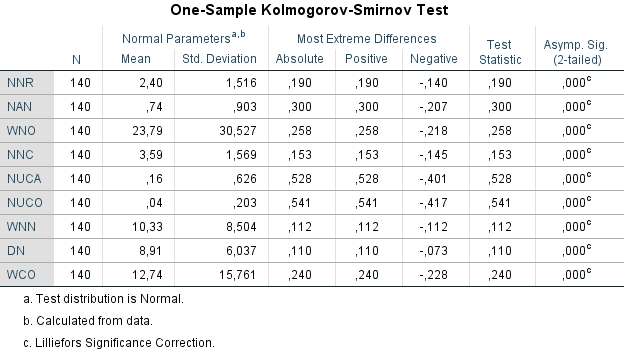
\includegraphics[width=0.48\textwidth]{figures/6_Results/Section2/01_KS_OCLmetrics}
\caption{Kolmogorov–Smirnov test on the normal distribution of OCL Complexity metrics}
\label{fig:01_ks_oclmetrics}
\end{figure}

% Hypothesis (intermediate): proposed metrics have a great deal of overlapping / reduced explanatory power

% Hypothesis: the learning outcome depends on OCL complexity and students proficiency

%In this section we present the analysis of the influence of OCL complexity on the success rate of student's assessments, as well as the influence of Natural Language complexity on the same outcome.

%Can OCL complexity explain the learning success rate? 

%Which metrics are relevant to explain that success? Since many metrics were proposed in the literature we must produce a variable reduction, not to obtain an overspecified model. To do so we started by doing a correlation analysis among the complexity metrics described in section~\ref{OCLComprehension}.

%First we assessed the normality of all those metrics, using a Kolmogorov-Smirnov test. The result in figure \ref{fig:01_ks_oclmetrics} indicates that the proposed OCL metrics do not follow a normal distribution, D(233) = 0.07, p = 0.005.

%KS results in APA style

%Which has more correlation with success?

To evaluate if the complexity of OCL expression (answers) can explain the success of students answers, and because the independent variables (metrics) don't follow a normal distribution, we applied a Spearman's rho correlation coefficient to evaluate their correlation, and their effect on the dependent variable (student's success). Figure~\ref{fig:01_sr_oclmetrics} presents the result of this assessment. We decided to exclude metrics with strong correlation (painted with red), as they can be used to explain the same results and keep the ones that are more dissimilar. The resulting metrics were NAN, WNO, NUCO, and WCO, as they revealed greater influence on the dependent variable.

\begin{figure}[!h]
\centering
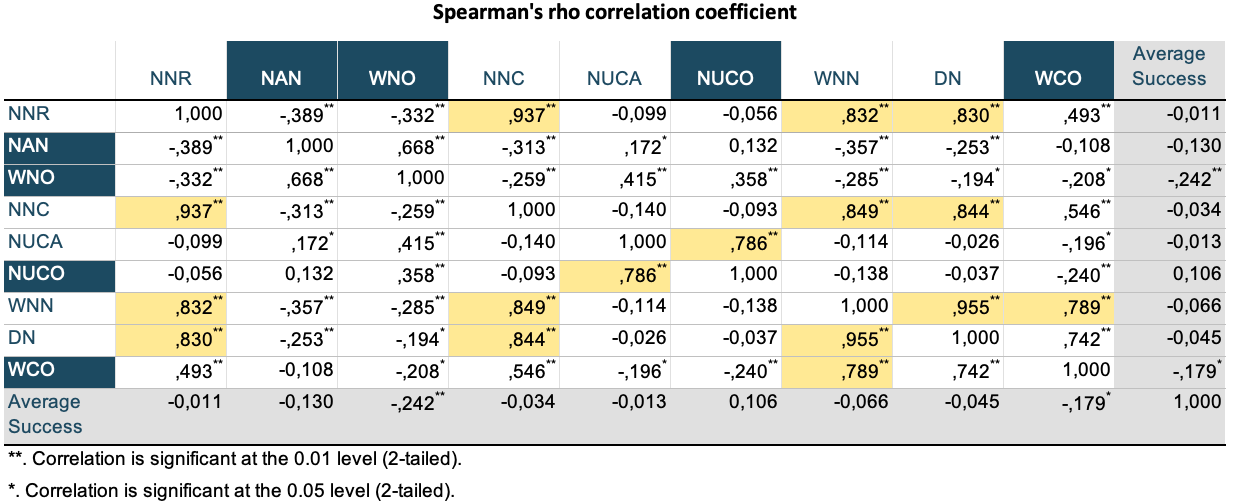
\includegraphics[width=0.48\textwidth]{figures/6_Results/Section2/01_SR_OCLmetrics}
\caption{Spearman's rho correlation coefficient of OCL Complexity metrics}
\label{fig:01_sr_oclmetrics}
\end{figure}

A similar study was applied to Natural Language metrics~\cite{readable}, which were calculated for each question. As many metrics were proposed, we must assemble a variable reduction, again to prevent an overspecific model. We started by assessing the normality of the given metrics, using a Kolmogorov-Smirnov test. The results in Figure~\ref{fig:02_ks_nlmetrics} indicates that the majority of the proposed Natural Language metrics do not follow a normal distribution, D(140) = .089, p = .009 (for Flesch–Kincaid Grade Level metric, other metrics show similar results).

\begin{figure}[!h]
\centering
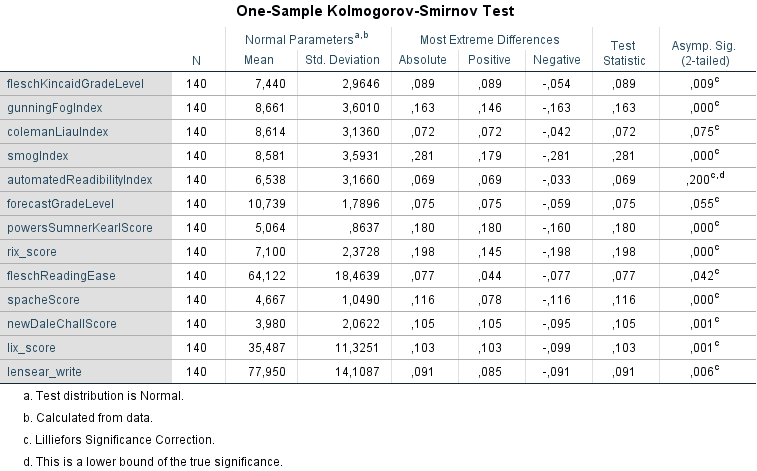
\includegraphics[width=0.49\textwidth]{figures/6_Results/Section2/02_KS_NLmetrics}
\caption{Kolmogorov–Smirnov test on the normal distribution of Natural Language metrics (English)}
\label{fig:02_ks_nlmetrics}
\end{figure}

To evaluate if the complexity of Natural Language (questions) can explain the success of students answers, and because the independent variables (metrics) don't follow a normal distribution, we applied a Spearman's rho correlation coefficient to evaluate their correlation, and their effect on the dependent variable (student's success). Figure~\ref{fig:02_sr_nlmetrics} presents the result of this assessment. We decided to exclude metrics with strong correlation (painted with red), as they can be used to explain the same results and keep the ones that are more dissimilar. The resulting metrics were the Automated Readability Index, Forest Grade Level, New Dale-Chall, and Lensear Write, as they revealed greater influence on the dependent variable.

\begin{figure}[!h]
\centering
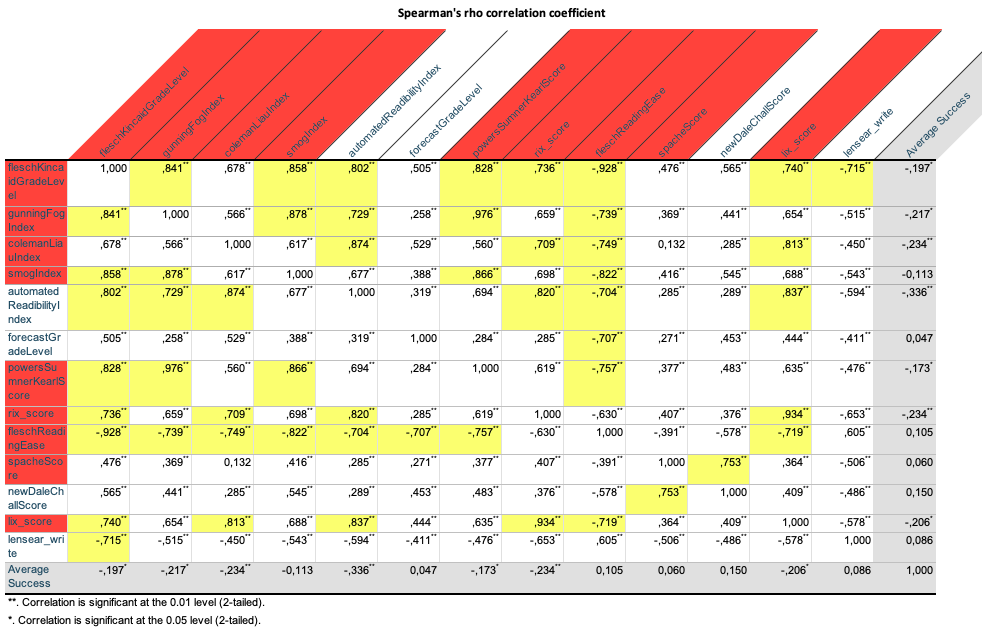
\includegraphics[width=0.49\textwidth]{figures/6_Results/Section2/02_SR_NLmetrics}
\caption{Spearman's rho correlation coefficient of NL metrics (English)}
\label{fig:02_sr_nlmetrics}
\end{figure}

Finally, after reducing the OCL and Natural Language metrics, we performed a Linear Regression to assess the capability of those metrics to explain the success of students, as Spearman's rho can evaluate relative monotonies whether the models are linear or not.

The results of the regression on OCL metrics are shown in Figure~\ref{fig:01_lr_oclmetrics}. A significant regression equation was found F(4, 135) = 4.313, $p<.01$, with an $R^{2}$ of .113.

\begin{figure}[!h]
\centering
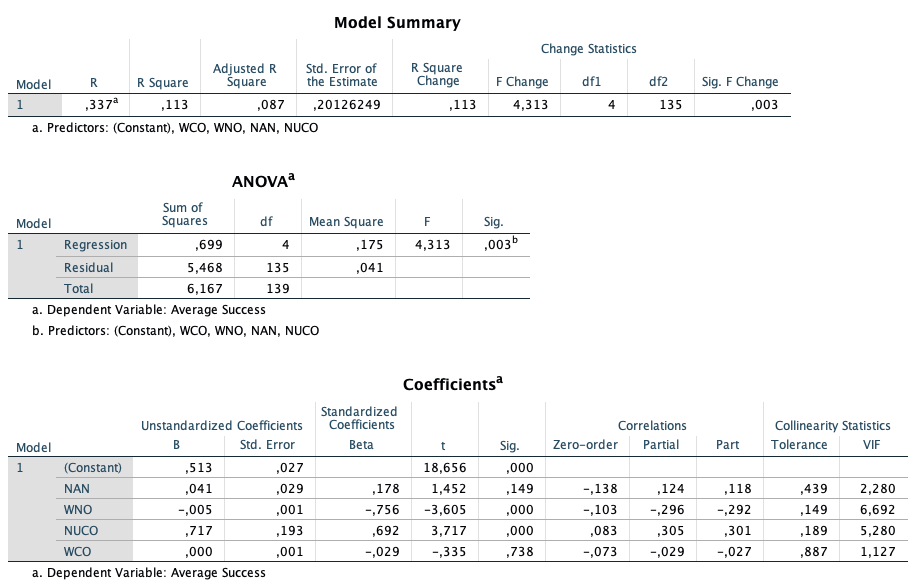
\includegraphics[width=0.49\textwidth]{figures/6_Results/Section2/01_LR_OCLmetrics.png}
\caption{Linear Regression using NAN, WNO, NUCO, and WCO to explain the success}
\label{fig:01_lr_oclmetrics}
\end{figure}

The results of the regression on Natural Language metrics are shown in Figure~\ref{fig:02_lr_nlmetrics}. A significant regression equation was found F(4, 135) = 6.311, $p<.001$, with an $R^{2}$ of .158.

\begin{figure}[!h]
\centering
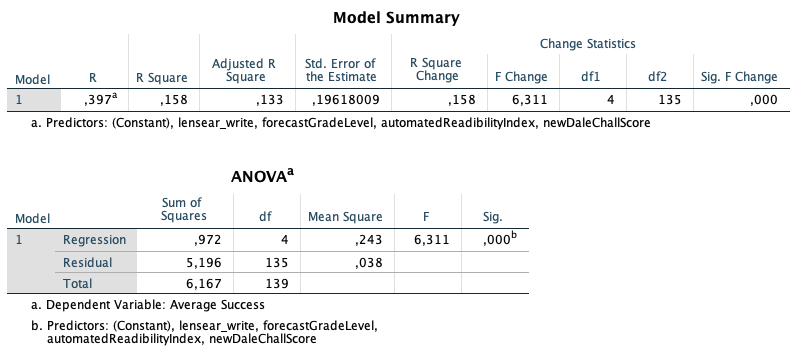
\includegraphics[width=0.48\textwidth]{figures/6_Results/Section2/02_LR_NLmetrics.png}
\caption{Linear Regression using Automated Readability Index, Forest Grade Level, New Dale-Chall, and Lensear Write to explain the success}
\label{fig:02_lr_nlmetrics}
\end{figure}

The resulting linear model in both cases (OCL and Natural Language metrics) revealed a poor explanatory power on the dependent variable, meaning that there is a monotony relationship, but it is not linear.
\end{comment}  